% == == == == == == == == == == == == == == == ==
%
%   A sample latex file for UoY, Dept. Electronics
%   Lab reports. This is NOT an official document
%   Just some thing I find useful when starting a
%   lab report in latex.
%
%   By  Zak R. A. West, zraw500@york.ac.uk
%
%   Licensed under the GNU GPL v2.0 license
%
% == == == == == == == == == == == == == == == ==

% Use the article class with font size 11pt
\documentclass[10pt]{article}

% Creates placeholder text (Only needed for this example)
\usepackage{blindtext}

% Deal with language and encoding
\usepackage[T1]{fontenc}
\usepackage[utf8]{inputenc}
\usepackage[english]{babel}

% setup page size
\usepackage{geometry}
\geometry{a4paper,margin=1.5in,lmargin=1in,rmargin=1in} % reduced margins

% Set up fancy headers and footers
\usepackage{fancyhdr} 
\pagestyle{fancy} % options: empty , plain , fancy
\renewcommand{\headrulewidth}{1pt} % adds line at the bottom of the header

% Set up table of contents
\usepackage[nottoc,notlof,notlot]{tocbibind}
\usepackage[titles,subfigure]{tocloft}

% Set up graphics and figures
\usepackage{graphicx}
\usepackage{wrapfig}
\usepackage{subfig}

% Better tables in latex
\usepackage[table,xcdraw]{xcolor}
\usepackage{booktabs} 
\usepackage{multirow}

% Begin paragraphs with an empty line rather than an indent
\usepackage[parfill]{parskip}

% For including code 
%\usepackage{verbatim}
\usepackage{listings}
\usepackage{color}

% Setup colors for code highlighting
\definecolor{commentcolor}{rgb}{0,0.4,0}
\definecolor{stringcolor}{rgb}{0.5,0.8,0.5}
\definecolor{identifiercolor}{rgb}{0.1,0.1,0.1}
\definecolor{keywordcolor}{rgb}{0.2,0,0.9}

\definecolor{numbercolor}{rgb}{0.5,0.5,0.5}
\definecolor{backgroundcolor}{rgb}{0.975,0.975,0.975}

% Setup style of code listings
\lstset{
    breakatwhitespace=false,
    breaklines=true,
    commentstyle=\itshape\color{commentcolor},
    frame=leftline,
    backgroundcolor=\color{backgroundcolor},
    keepspaces=true,
    keywordstyle=\bfseries\color{keywordcolor},
    identifierstyle=\color{identifiercolor},
    numbers=left,
    numbersep=10pt,
    numberstyle=\small\color{numbercolor},
    rulecolor=\color{black},
    showspaces=false,
    showstringspaces=false,
    showtabs=false,
    stepnumber=1,
    stringstyle=\color{stringcolor},
    tabsize=2,
    title=\lstname
}

% Better maths rendering
\usepackage{array}

% For more list types
\usepackage{paralist}

% Better section formatting
\usepackage{sectsty}

% Sets up formatting for section headings
\allsectionsfont{\sffamily\mdseries\upshape}
\renewcommand{\cftsecfont}{\rmfamily\mdseries\upshape}
\renewcommand{\cftsecpagefont}{\rmfamily\mdseries\upshape}

% Set up header and footer text
\makeatletter
\lhead{\@title}\chead{}\rhead{\@author}
\lfoot{}\cfoot{\thepage}\rfoot{}
\makeatother

% Should show blue underlines on links, but it doesn't appear to work
\usepackage[colorlinks=false, allbordercolors={0 0 0}, linkbordercolor=blue, pdfborderstyle={/S/U/W 1}]{hyperref}

% Tell latex that your images are in a folder called Images
\graphicspath{{Images/},{tables/}}

% Use url for better url handling
\usepackage{url}

% Use biblatex for citations
\usepackage{csquotes}
\usepackage[
    backend=biber,
    style=numeric,
    sorting=ynt
]{biblatex}
\addbibresource{references.bib}

% My custom title page package
\usepackage{UoYTitlePage}


%%% =====================================================
%%% =====================================================
%%%     You Should Only Have To Edit Stuff Below
%%%     Here. Unless You Want To Change The Style.
%%% =====================================================
%%% =====================================================


% ====================================
% Set up tile, author and other stuff
% ====================================

\uni{University of York}
\dept{Department of Electronics}

\module{Computer Architectures}
\project{Homework One}

\title{Homework One}
\author{Y3839090}

\supervisor{ }
\logo{logo}

\abstracttext{
	Homework one for Computer Architectures module.
}

% ====================================
% Start of the main document
% ====================================
\begin{document}
    
	% ============
	% Title Page
	% ============
	\maketitle
	
	% ============
	% Contents Page
	% ============
	\pagenumbering{roman} % Use roman numerals for page numbers
	\tableofcontents % Adds a table of contents
	\listoffigures % Adds a list of figures
	\newpage
	\pagenumbering{arabic} % Use Arabic (integer) numbering

	% ============
	% Main Pages
	% ============
	\section{Question 1}
		\subsection{Extra Instructions}
        
        The current instruction set for architecture B is lacking the XOR and AND instructions. These are both logic instructions so they will be grouped with the other logic instructions. This means there opcodes will start with 01 (the same as the other logic instructions). Both of these instruction take the three operands Rt, Ra and Rb and so will use the same instruction coding as the ADD and SUB instructions (ADD and SUB also take Rt, Ra and Rb operands).
        
\begin{table}[ht]
\centering
\caption{The extra instructions need for Arch B to run the program}
\label{table:extrainstructions}
\begin{tabular}{l|lll}
\rowcolor[HTML]{417CB4} 
{\color[HTML]{FFFFFF} \textbf{Command}} & {\color[HTML]{FFFFFF} \textbf{Operands}} & {\color[HTML]{FFFFFF} \textbf{Opcode}} & {\color[HTML]{FFFFFF} \textbf{Fields}} \\ \hline
\rowcolor[HTML]{C4D9E1} 
\cellcolor[HTML]{417CB4}{\color[HTML]{FFFFFF} and} & Rt, Ra, Rb & 01 100 & xxx xxxx xBBB xxxx xAAA xxxx xTTT \\
\rowcolor[HTML]{DBE5E8} 
\cellcolor[HTML]{417CB4}{\color[HTML]{FFFFFF} xor} & Rt, Ra, Rb & 01 110 & xxx xxxx xBBB xxxx xAAA xxxx xTTT
\end{tabular}
\end{table}

		\subsection{Conversions}
        
        	\subsubsection{Assembly}
            
            	This is the given pseudo code converted to the assembly language defined for architecture B.
            	\lstinputlisting[language={[x86masm]Assembler},title={Assembly code}]{code/assembly.txt}
                \vspace{1cm}

             \subsubsection{Machine code - Binary}
             
             	This is the above assembly code hand assembled into binary. ``x" has been used to represent ``don't care'' bits.
             	\lstinputlisting[language={[x86masm]Assembler},title={Machine code - Binary with don't cares}]{code/MachineCodeBinaryx.txt}
               
               To be able to convert this to hex, the “don’t care” bits have to changed to either 0 or 1. I decided to convert all of the ``dont care'' bits to 0’s.
               
               \lstinputlisting[language={[x86masm]Assembler},title={Machine code - Binary, don't cares replace with 0s}]{code/MachineCodeBinary.txt}

             \subsubsection{Machine code - Hex}
             
             This is the above binary machine code shown as hexadecimal. Remember all “don’t cares” have been converted to zero so that the values can be represented in hex.
             
				\lstinputlisting[language={[x86masm]Assembler},title={Machine code - Hex, don't cares replace with 0s}]{code/MachineCodeHex.txt}
                
     	\subsection{Control Signals}
		
		Here is a table of all the necessary control signals needed to run the given program on Architecture B.
		\begin{figure}[ht]
          			\centering
          			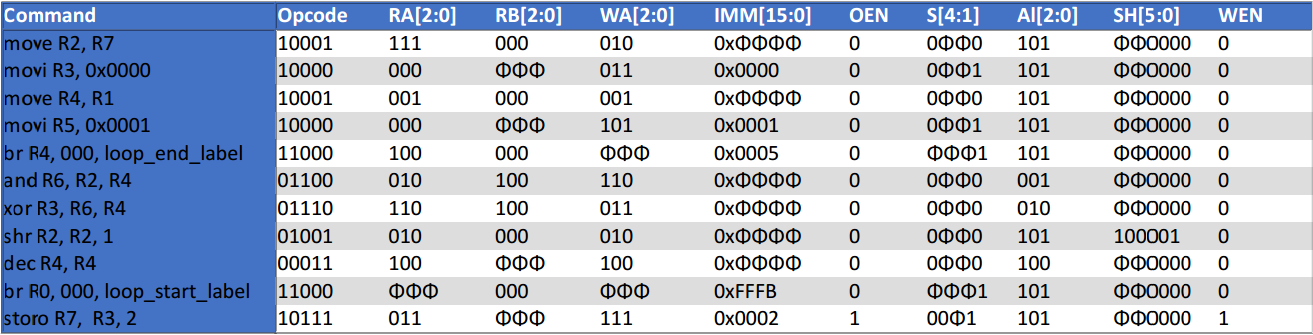
\includegraphics[width=1\textwidth]{tables/Q1ControlSignals}
          			\caption{Control signals}
         		\end{figure}

\newpage

\section{Question 2}
    	
        Here is a table showing all the control signals need to execute the instruction with the multi-cycle architecture C.
    
        \begin{figure}[ht]
          \centering
          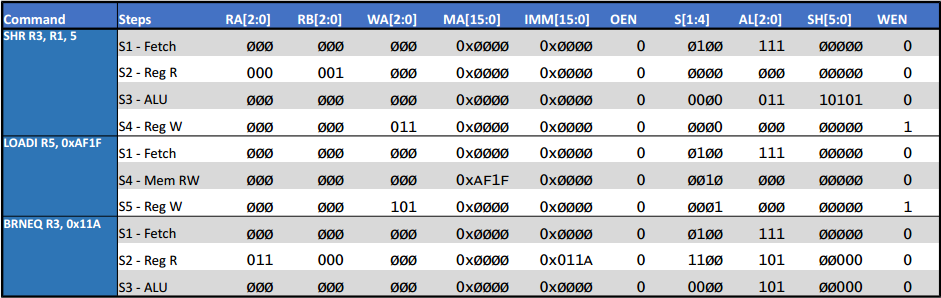
\includegraphics[width=1\textwidth]{tables/Q2ControlSignals}
          \caption{Stages and control signals}
        \end{figure}
        
        
	\section{Question 3}
    
    Here is my encoding for each of the instructions in the set.
    
    \begin{figure}[ht]
      \centering
      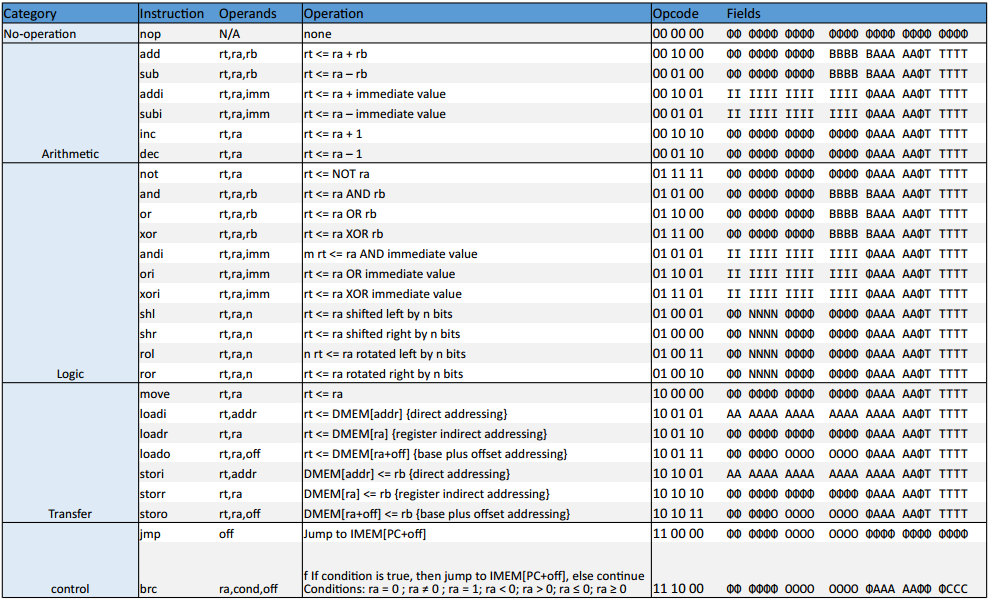
\includegraphics[width=1\textwidth]{tables/InstructionSet}
      \caption{Instruction set encoding}
    \end{figure}

	
    % ============
	% Bibliography Pages
	% ============
	\newpage
	\printbibliography
	\newpage
	
% ============
% Appendix Pages
% ============
%   \appendix
%  \section*{Appendices}
%   \addcontentsline{toc}{section}{Appendices}
%    \renewcommand{\thesubsection}{\Alph{subsection}}
    
    % Add appendices here as subsections
    
    
            
         
    
    
\end{document}